% !TeX encoding = UTF-8
% !TeX root = ../main.tex

%% ------------------------------------------------------------------------
%% Copyright (C) 2021 SJTUG
%% 
%% SJTUBeamer Example Document by SJTUG
%% 
%% SJTUBeamer Example Document is licensed under a
%% Creative Commons Attribution-NonCommercial-ShareAlike 4.0 International License.
%% 
%% You should have received a copy of the license along with this
%% work. If not, see <http://creativecommons.org/licenses/by-nc-sa/4.0/>.
%% -----------------------------------------------------------------------

\section{Background}

\subsection{Motivation}

\begin{frame}{Motivation}
	\begin{block}{Goal}
        Applying ML to systems (blockchain-based models)
      \end{block}
  \begin{itemize}
    \item Research interest mainly targeted to \alert{blockchain technology}
    \item Research group in Department of Automation (PhD supervisors) has been recently working in blockchain-based models for \alert{trust management systems}
	\item Specifically, applied to data-aggregation systems in the Internet of Things (IoT) field (crowdsensing)
	\item Could similar approach be applied for \alert{Federated Learning}?
%    \item My PhD thesis could use some of the model simulation techniques (stochastic processes) used in this research paper experimentation
%    \item And of course, it is related to a emerging subfield that could greatly contribute to the development of the Internet of Things (IoT)
  \end{itemize}
\end{frame}

\subsection{Blockchain technology}

\begin{frame}{Blockchain background}
  \alert{Distributed ledger containing a time-stamped series of immutable blockchains, trustless, decentralized, proof-tampering and full traceability}
  \begin{itemize}
    \item Research approaches on blockchain-based Federated Learning:
          \begin{itemize}
            \item Evaluating time consumption and task cost of applying a blockchain-based system%\cite{paper33}
            \item Blockchain-based crowdsourcing quality control model%\cite{paper34}
            \item Considering privacy issues%\cite{paper35}
            \item Handling location privacy protection%\cite{paper37} (confusion mechanism)
          \end{itemize}
  \end{itemize}
\end{frame}

\subsection{Crowdsourcing}

\begin{frame}{Crowdsourcing: definition}
  \begin{itemize}
  \item \textbf{Crowdsourcing:} emerging paradigm of data aggregation, having a key role in data-driven applications. Actors involved sometimes work as paid freelancers, while others perform tasks voluntarily.
  \item \textbf{Benefit:} improved data collection efficiency and reduced costs effectively%\cite{paper2}
  \item Incentive-aware Federated Learning is linked to crowdsourcing theory (contest \& auction theory)
  \end{itemize}
  \begin{figure}[h]
        \centering
        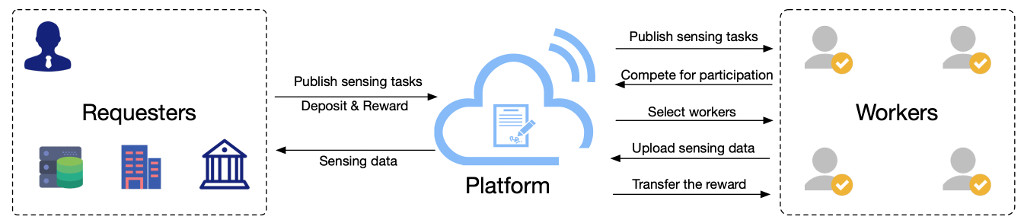
\includegraphics[width=.8\textwidth]{201909-wei-figure1.jpg}
      \end{figure}
\end{frame}

\begin{frame}{Crowdsourcing: issues}
  		\begin{enumerate}
   			\item Managed and maintained \alert{centralized platforms} suffer from the single point of failure
   				\begin{itemize}
   					\item \textbf{Solution: } decentralized architecture (blockchain technology) that lacks a single point of failure, and enhances privacy with asymmetric encryption and digital signature technology
   				\end{itemize}
    		\item Encouraging workers by offering appropiate \alert{incentive mechanisms} (monetary usually) \rightarrow  \underline{auction theory} guarantees benefits for both requesters and workers\cite{electronics9020215} but only provide short-term incentives
    			\begin{itemize}
   					\item \textbf{Solution:} hybrid incentive mechanism, adopting \underline{mechanism design theory}, considering three factors:
   					\begin{itemize}
   					\item Monetary reward
   					\item Reputation evaluation
   					\item Data quality
   					\end{itemize}
   				\end{itemize}
  		\end{enumerate}
\end{frame}